\documentclass{standalone}
\usepackage{tikz,pgfplots}
\usetikzlibrary{calc}

\pgfplotsset{%
    compat=newest, %footnotesize
    tick label style={font=\footnotesize},
    label style={font=\small},
    legend style={font=\small},
    axis x line = center,
    axis y line = center,
    every axis/.style={pin distance=1ex}
    cmhplot/.style={color=black,mark=none,line width=1pt,->},
    soldot/.style={color=black,only marks,mark=*},
    coldot/.style={color=black,fill=white,only marks,mark=*},
}


\begin{document}
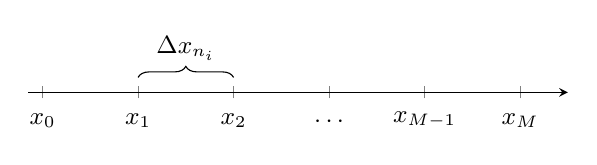
\begin{tikzpicture}
\begin{axis}[%
axis x line=center,
axis y line=none,ymin=-1.5,ymax=1.5,
xmin=-0.03,xmax=1.1,
xticklabel=\empty
]
\node[black,above] at (axis cs:0.0,-0.3){\small{$x_0$}};
\node[black,above] at (axis cs:0.2,-0.3){\small{$x_1$}};
\node[black,above] at (axis cs:0.4,-0.3){\small{$x_2$}};
\node[black,above] at (axis cs:0.6,-0.3){\small{$\cdots$}};
\node[black,above] at (axis cs:0.8,-0.3){\small{$x_{M-1}$}};
\node[black,above] at (axis cs:1.0,-0.3){\small{$x_M$}};
\node[black,above] at (axis cs:0.3,0.15){\small{$\Delta x_{n_i}$}};

\draw [decorate,decoration={brace,amplitude=4pt}]
(0.2,0.1)--(0.4,0.1) node[midway, above, font=\footnotesize, xshift=2pt] {};


\end{axis}
\end{tikzpicture}


\end{document}